%% Espaço Mental M: O Campo Vetorial da Mente em R^15

\chapter{O Espaço Mental $\mathcal{M}$: Definições e Estrutura}

\epigrafe{A mente humana é um espaço de infinitas dimensões, mas podemos capturar sua essência em coordenadas fundamentais.}{Gustavo Mendes e Silva}

\section{Introdução ao Espaço Mental}

O Espaço Mental $\mathcal{M}$ é uma estrutura matemática que representa a mente humana como um campo vetorial em $\mathbb{R}^{15}$. Esta formalização permite:
\begin{itemize}
    \item Quantificar estados mentais de forma precisa
    \item Rastrear trajetórias emocionais e cognitivas
    \item Validar intervenções terapêuticas matematicamente
    \item Integrar múltiplos frameworks psicológicos estabelecidos
\end{itemize}

\section{Os 15 Vetores-Dimensões do Espaço Mental}

O espaço $\mathcal{M} \subset \mathbb{R}^{15}$ é definido pelas seguintes dimensões, cada uma validada por frameworks científicos estabelecidos:

\begin{center}
\begin{tikzpicture}[scale=0.9]
    % Círculo central
    \node[draw, circle, fill=yellow!40, minimum size=3cm, font=\large\bfseries] at (0,0) {$\mathcal{M}$};

    % 15 dimensões ao redor
    \foreach \i/\nome/\cor in {
        1/Valência/red,
        2/Excitação/orange,
        3/Dominância/yellow,
        4/Cognição/green,
        5/Abertura/teal,
        6/Conscienciosidade/blue,
        7/Extroversão/purple,
        8/Amabilidade/pink,
        9/Neuroticismo/gray,
        10/Positividade/lime,
        11/Engajamento/cyan,
        12/Significado/violet,
        13/Funcionalidade/brown,
        14/Linguagem/magenta,
        15/Temporalidade/olive
    } {
        \pgfmathsetmacro{\angle}{90 - (\i-1)*24}
        \node[draw, rounded corners, fill=\cor!20, font=\tiny, text width=1.3cm, align=center]
            at (\angle:4.5) {$v_{\i}$\\\nome};
        \draw[thick, ->, \cor!60] (\angle:2) -- (\angle:3.8);
    }
\end{tikzpicture}
\end{center}

\subsection{Dimensões Emocionais (1-3): Validação pelo Modelo PAD}

Baseadas no modelo PAD (Pleasure-Arousal-Dominance) de Mehrabian e Russell:

\begin{equation}
\vec{v}_{\text{emocional}} = (v_1, v_2, v_3) \in [-1, 1]^3
\end{equation}

\begin{itemize}
    \item $v_1$ --- \textbf{Valência} (Pleasure): Grau de prazer ou desprazer
    \item $v_2$ --- \textbf{Excitação} (Arousal): Nível de ativação fisiológica
    \item $v_3$ --- \textbf{Dominância} (Dominance): Senso de controle
\end{itemize}

\subsection{Dimensões Cognitivas (4): Validação pelo RDoC}

Baseado no Research Domain Criteria (RDoC) do NIMH:

\begin{equation}
v_4 \in [0, 1]: \text{Capacidade de Processamento Cognitivo}
\end{equation}

Inclui atenção, memória de trabalho, controle cognitivo e flexibilidade.

\subsection{Dimensões de Personalidade (5-9): Validação pelo Big Five (OCEAN)}

O modelo de Cinco Grandes Fatores (Big Five):

\begin{equation}
\vec{v}_{\text{personalidade}} = (v_5, v_6, v_7, v_8, v_9) \in [0, 1]^5
\end{equation}

\begin{itemize}
    \item $v_5$ --- \textbf{Abertura} (Openness): Criatividade e curiosidade
    \item $v_6$ --- \textbf{Conscienciosidade} (Conscientiousness): Organização e disciplina
    \item $v_7$ --- \textbf{Extroversão} (Extraversion): Sociabilidade e energia
    \item $v_8$ --- \textbf{Amabilidade} (Agreeableness): Cooperação e empatia
    \item $v_9$ --- \textbf{Neuroticismo} (Neuroticism): Instabilidade emocional
\end{itemize}

\subsection{Dimensões de Bem-Estar (10-12): Validação pelo PERMA}

Modelo PERMA de Martin Seligman:

\begin{equation}
\vec{v}_{\text{bem-estar}} = (v_{10}, v_{11}, v_{12}) \in [0, 1]^3
\end{equation}

\begin{itemize}
    \item $v_{10}$ --- \textbf{Positividade} (Positive Emotions): Emoções positivas
    \item $v_{11}$ --- \textbf{Engajamento} (Engagement): Estado de fluxo
    \item $v_{12}$ --- \textbf{Significado} (Meaning): Propósito e sentido
\end{itemize}

\subsection{Dimensão Funcional (13): Validação pelo WHODAS 2.0}

Baseado no WHO Disability Assessment Schedule:

\begin{equation}
v_{13} \in [0, 1]: \text{Funcionalidade Global}
\end{equation}

Avalia capacidade de funcionamento em domínios da vida diária.

\subsection{Dimensão Linguística (14): Central ao Tratado}

\begin{equation}
v_{14} \in [0, 1]: \text{Coerência e Organização Linguística}
\end{equation}

Medida central do tratado, refletindo integração cognitivo-emocional.

\subsection{Dimensão Temporal (15): Orientação no Tempo}

\begin{equation}
v_{15} \in [-1, 1]: \text{Foco Temporal} \quad (\text{passado} \to \text{futuro})
\end{equation}

Indica orientação predominante: ruminação (passado) ou planejamento (futuro).

%% Integração com HiTOP
\section{Integração com o Modelo HiTOP}

O Hierarchical Taxonomy of Psychopathology (HiTOP) organiza a psicopatologia em espectros dimensionais. Nosso espaço $\mathcal{M}$ se conecta ao HiTOP através de:

\begin{center}
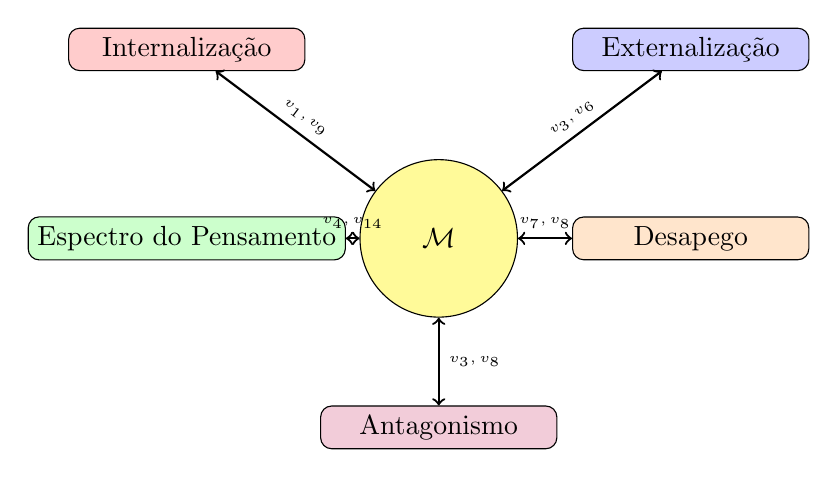
\begin{tikzpicture}[scale=0.8]
    % Espectros HiTOP
    \node[draw, rounded corners, fill=red!20, minimum width=3cm] (int) at (-4,3) {Internalização};
    \node[draw, rounded corners, fill=blue!20, minimum width=3cm] (ext) at (4,3) {Externalização};
    \node[draw, rounded corners, fill=green!20, minimum width=3cm] (tho) at (-4,0) {Espectro do Pensamento};
    \node[draw, rounded corners, fill=orange!20, minimum width=3cm] (det) at (4,0) {Desapego};
    \node[draw, rounded corners, fill=purple!20, minimum width=3cm] (ant) at (0,-3) {Antagonismo};

    % Espaço M central
    \node[draw, circle, fill=yellow!40, minimum size=2cm] (M) at (0,0) {$\mathcal{M}$};

    % Conexões
    \draw[thick, <->] (int) -- node[above, sloped, font=\tiny] {$v_1, v_9$} (M);
    \draw[thick, <->] (ext) -- node[above, sloped, font=\tiny] {$v_3, v_6$} (M);
    \draw[thick, <->] (tho) -- node[above, sloped, font=\tiny] {$v_4, v_{14}$} (M);
    \draw[thick, <->] (det) -- node[above, sloped, font=\tiny] {$v_7, v_8$} (M);
    \draw[thick, <->] (ant) -- node[right, font=\tiny] {$v_3, v_8$} (M);
\end{tikzpicture}
\end{center}

\chapter{Visualizações de Estados Mentais}

\section{Representação de um Estado Mental}

Um estado mental $\psi \in \mathcal{M}$ é um vetor:

\begin{equation}
\psi = (v_1, v_2, v_3, v_4, v_5, v_6, v_7, v_8, v_9, v_{10}, v_{11}, v_{12}, v_{13}, v_{14}, v_{15})
\end{equation}

\subsection{Exemplo: Estado de Depressão}

\begin{center}
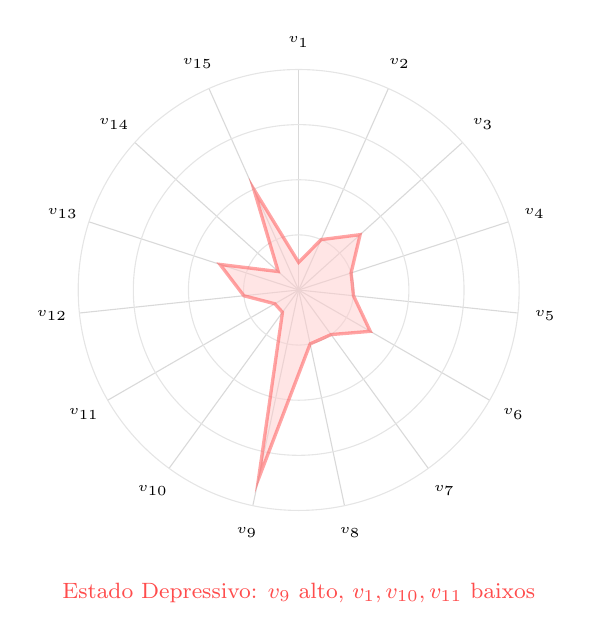
\begin{tikzpicture}[scale=0.7]
    % Radar chart
    \foreach \i in {1,...,15} {
        \pgfmathsetmacro{\angle}{90 - (\i-1)*24}
        \draw[gray!30] (0,0) -- (\angle:4);
        \node[font=\tiny] at (\angle:4.5) {$v_{\i}$};
    }

    % Círculos de referência
    \draw[gray!20] (0,0) circle (1);
    \draw[gray!20] (0,0) circle (2);
    \draw[gray!20] (0,0) circle (3);
    \draw[gray!20] (0,0) circle (4);

    % Estado depressivo (valores baixos em positivos, altos em neuroticismo)
    \draw[very thick, red!70, fill=red!20, opacity=0.5]
        (90:0.5) -- (66:1) -- (42:1.5) -- (18:1) -- (-6:1) -- (-30:1.5) --
        (-54:1) -- (-78:1) -- (-102:3.5) -- (-126:0.5) -- (-150:0.5) --
        (-174:1) -- (-198:1.5) -- (-222:0.5) -- (-246:2) -- cycle;

    \node[font=\footnotesize, red!70] at (0,-5.5) {Estado Depressivo: $v_9$ alto, $v_1, v_{10}, v_{11}$ baixos};
\end{tikzpicture}
\hspace{1cm}
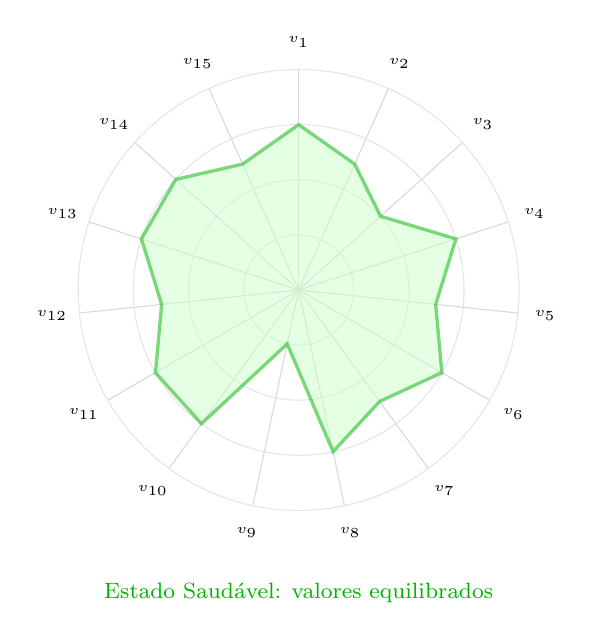
\begin{tikzpicture}[scale=0.7]
    % Radar chart
    \foreach \i in {1,...,15} {
        \pgfmathsetmacro{\angle}{90 - (\i-1)*24}
        \draw[gray!30] (0,0) -- (\angle:4);
        \node[font=\tiny] at (\angle:4.5) {$v_{\i}$};
    }

    % Círculos de referência
    \draw[gray!20] (0,0) circle (1);
    \draw[gray!20] (0,0) circle (2);
    \draw[gray!20] (0,0) circle (3);
    \draw[gray!20] (0,0) circle (4);

    % Estado saudável (valores equilibrados)
    \draw[very thick, green!70!black, fill=green!20, opacity=0.5]
        (90:3) -- (66:2.5) -- (42:2) -- (18:3) -- (-6:2.5) -- (-30:3) --
        (-54:2.5) -- (-78:3) -- (-102:1) -- (-126:3) -- (-150:3) --
        (-174:2.5) -- (-198:3) -- (-222:3) -- (-246:2.5) -- cycle;

    \node[font=\footnotesize, green!70!black] at (0,-5.5) {Estado Saudável: valores equilibrados};
\end{tikzpicture}
\end{center}

\section{Trajetórias no Espaço Mental}

A evolução temporal de um estado mental descreve uma trajetória $\gamma(t)$ em $\mathcal{M}$:

\begin{equation}
\gamma: [t_0, t_f] \to \mathcal{M}, \quad \gamma(t) = \psi(t)
\end{equation}

A \textbf{velocidade de mudança} é dada por:

\begin{equation}
\frac{d\psi}{dt} = \left(\frac{dv_1}{dt}, \frac{dv_2}{dt}, \ldots, \frac{dv_{15}}{dt}\right)
\end{equation}

\begin{center}
\begin{tikzpicture}[scale=1]
    % Eixos simplificados (projeção 3D)
    \draw[thick, ->] (0,0) -- (5,0) node[right] {$v_1$ (Valência)};
    \draw[thick, ->] (0,0) -- (0,4) node[above] {$v_{10}$ (Positividade)};
    \draw[thick, ->] (0,0) -- (-2,-1.5) node[below left] {$v_{14}$ (Linguagem)};

    % Trajetória terapêutica
    \draw[very thick, blue!70, smooth, ->]
        plot coordinates {(1,1) (1.5,1.2) (2,1.8) (2.5,2.2) (3,2.5) (3.5,3) (4,3.2)};

    % Pontos marcados
    \fill[red] (1,1) circle (0.1) node[below left, font=\tiny] {início};
    \fill[green!70!black] (4,3.2) circle (0.1) node[above right, font=\tiny] {após terapia};

    % Seta de progresso
    \draw[thick, ->, orange] (2.5,0.5) -- (3.5,0.5) node[right, font=\footnotesize] {progresso};
\end{tikzpicture}
\end{center}

\section{Distância entre Estados Mentais}

A distância entre dois estados $\psi_1$ e $\psi_2$ em $\mathcal{M}$:

\begin{equation}
d(\psi_1, \psi_2) = \sqrt{\sum_{i=1}^{15} w_i (v_{1i} - v_{2i})^2}
\end{equation}

Onde $w_i$ são pesos que podem refletir a importância clínica de cada dimensão.

\chapter{Operações no Espaço Mental}

\section{Projeções e Subespaços}

Podemos projetar $\mathcal{M}$ em subespaços clinicamente relevantes:

\begin{align}
\pi_{\text{emocional}}: \mathcal{M} &\to \mathbb{R}^3, \quad \psi \mapsto (v_1, v_2, v_3) \\
\pi_{\text{Big5}}: \mathcal{M} &\to \mathbb{R}^5, \quad \psi \mapsto (v_5, v_6, v_7, v_8, v_9) \\
\pi_{\text{PERMA}}: \mathcal{M} &\to \mathbb{R}^3, \quad \psi \mapsto (v_{10}, v_{11}, v_{12})
\end{align}

\section{Transformações Terapêuticas}

Uma intervenção terapêutica $T$ pode ser modelada como uma transformação:

\begin{equation}
T: \mathcal{M} \to \mathcal{M}, \quad \psi_{\text{antes}} \mapsto \psi_{\text{depois}}
\end{equation}

O \textbf{efeito terapêutico} é medido por:

\begin{equation}
\Delta\psi = T(\psi) - \psi = \psi_{\text{depois}} - \psi_{\text{antes}}
\end{equation}

\section{Índice de Saúde Mental}

Um índice escalar de saúde mental pode ser definido:

\begin{equation}
H(\psi) = \frac{1}{15}\sum_{i=1}^{15} \alpha_i \cdot f_i(v_i)
\end{equation}

Onde $\alpha_i$ são pesos e $f_i$ são funções que mapeiam cada dimensão para uma contribuição ao bem-estar (considerando que algumas dimensões, como neuroticismo, contribuem negativamente).

\begin{sintese}[title=Síntese do Espaço Mental $\mathcal{M}$]
O Espaço Mental $\mathcal{M} \subset \mathbb{R}^{15}$ oferece uma estrutura matemática rigorosa para representar, analisar e intervir em estados mentais. Através da integração de frameworks validados (PAD, Big Five, PERMA, WHODAS, RDoC, HiTOP), este modelo permite:

\begin{itemize}
    \item Quantificar estados mentais multidimensionalmente
    \item Visualizar trajetórias terapêuticas
    \item Medir distâncias entre estados mentais
    \item Avaliar efeitos de intervenções
    \item Integrar linguagem, cognição e emoção em um framework unificado
\end{itemize}

A linguagem ($v_{14}$) ocupa posição central neste espaço, conectando-se a todas as outras dimensões e servindo como indicador e instrumento de transformação, conforme desenvolvido ao longo deste tratado.
\end{sintese}

\nextpage
